%! Author = Philipp Emmenegger
%! Date = 29/06/2021

\section{Security Testing}
Process intended to reveal flaws in the security mechanisms.\\
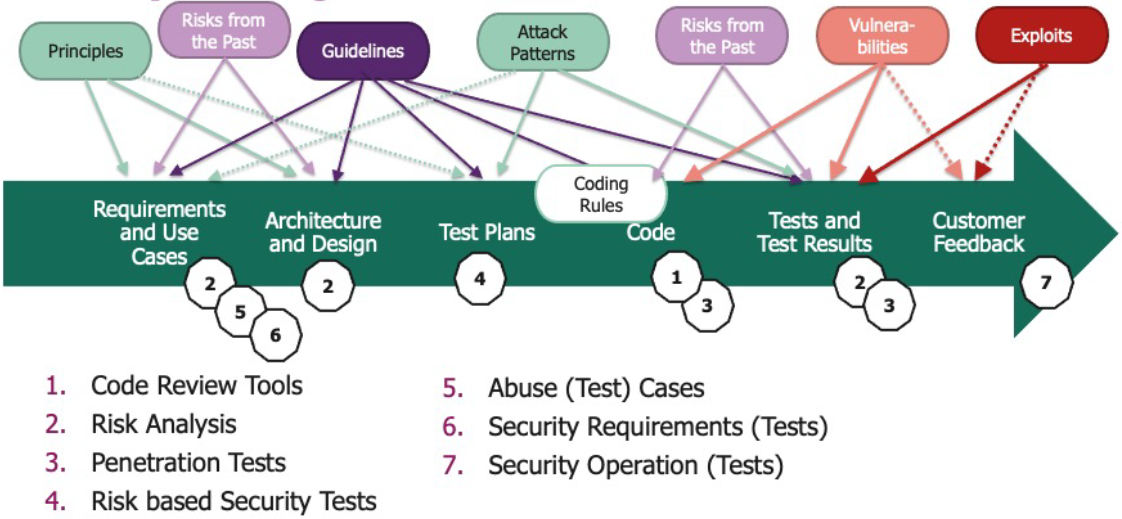
\includegraphics[width=\linewidth]{../img/security_testing.png}

\subsection{Verification in SDLC}
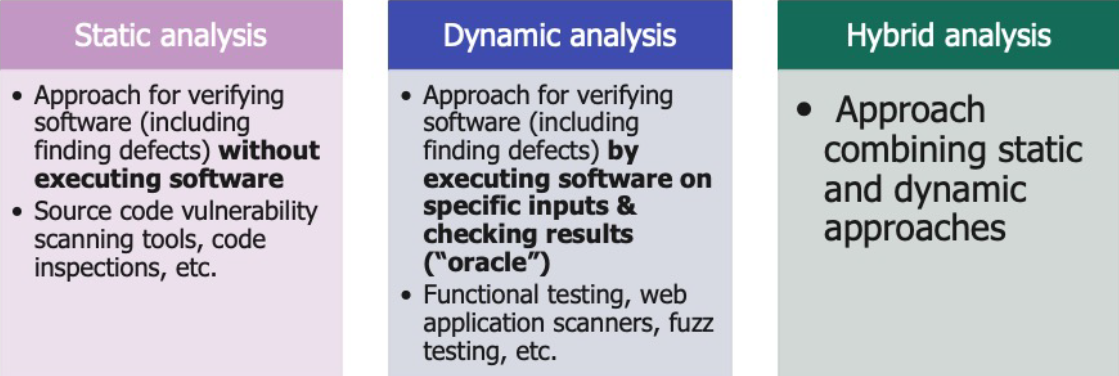
\includegraphics[width=\linewidth]{../img/verification_sdlc.png}

\subsection{Measurement Terminology}
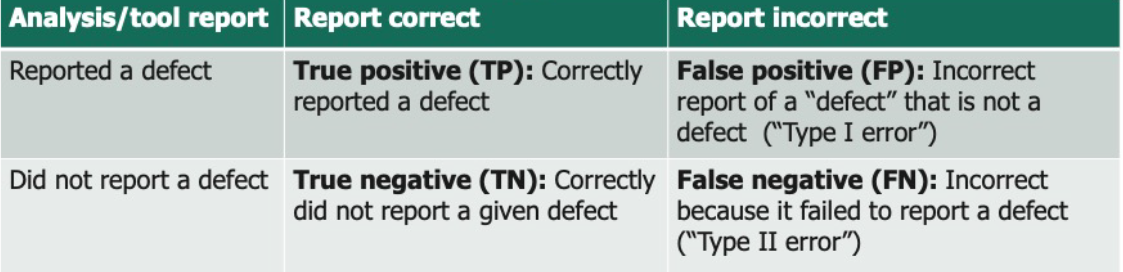
\includegraphics[width=\linewidth]{../img/measurement_terminology.png}
\textbf{Issues:}
\begin{itemize}
    \item Too many false positives: Tool wasted my time
    \item Too many false negatives: Tool missed the important
\end{itemize}

\subsection{Application to (Static) Application Security Testing Tools}
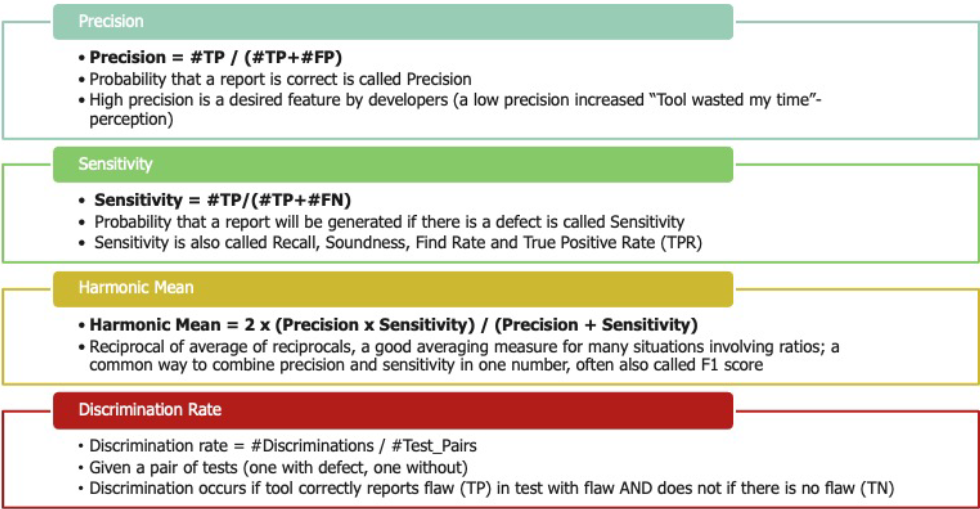
\includegraphics[width=\linewidth]{../img/application.png}

\columnbreak
\subsection{Static Analysis Tools}
\subsubsection{Static Application Security Testing (SAST)}
\begin{itemize}
    \item Based on white-hat / white-box
    \item Tester knows information about the system
    \item Examine source code at rest to detect and report security weaknesses
    \item Some tools run on source code, some on compiled code, some on both
\end{itemize}
\textbf{Functional Components of a SAST Tool}\\
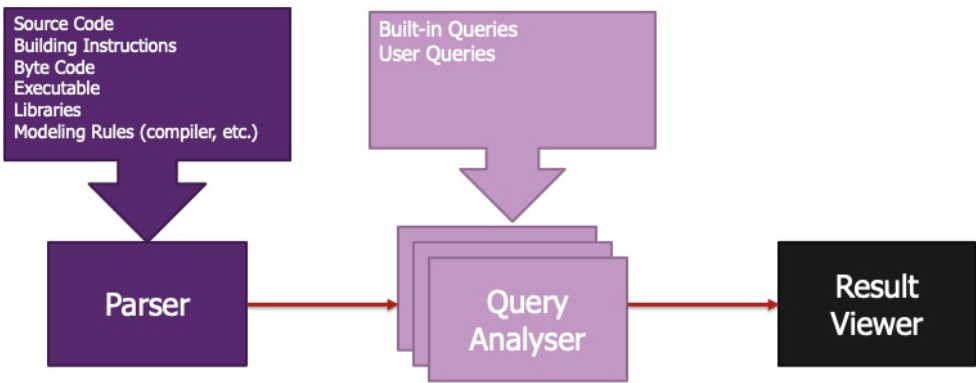
\includegraphics[width=\linewidth]{../img/sast_tool.png}\\
\textbf{Data Flow Analysis Techniques compiled into SAST}
\begin{enumerate}
    \item Control Flow Graph: Follow the control flow to identify dangerous sequences
    \item Tainting Analysis: Identify variable that have been tainted with user input, follow them if passed without sanitization
    \item Lexical Analysis: Tokenize source code to make it easier to analyse
\end{enumerate}

\subsection{Dynamic Analysis Tools}
\subsubsection{Web Application Scanners}
\begin{itemize}
    \item Pretend Browser
    \item Goes through the various web forms and links
    \item Sends in attack-like and random data, tries to detect problems
    \item Easy and quick to use
    \item OWASP ZAP
\end{itemize}

\subsubsection{Fuzzing}
\begin{itemize}
    \item Provide a large number of random inputs
    \item Monitor program results and not if the final answer is correct
    \begin{itemize}
        \item Crashes
        \item Fails code assertions
        \item Memory leaks
    \end{itemize}
\end{itemize}

\subsubsection{Test Data Creation Techniques}
\begin{enumerate}
    \item Black Box (fully random): Feed the program random inputs. Very easy but rather inefficient
    \item Mutation based: Mutate input samples to create test data
    \item Generation based: Create test data based on model of input
\end{enumerate}
\textbf{Imporvements:}
\begin{itemize}
    \item Constraints: Generating tests that execute previously unused code paths
    \item Heuristics: Create likely security vulnerability patterns
    \item Variate on the type of input data
\end{itemize}

\subsection{Code Coverage}
\begin{itemize}
    \item \textbf{Statement coverage:} Which percentage of statements have been executed
    \item \textbf{Branch coverage:} Which percentage of branch options have been executed
\end{itemize}

\subsection{Software Composition Analysis (SCA)}
\begin{itemize}
    \item Historically developed to check legal status of embedded software libraries
    \item Today: powerful tool to get inside about the propagation of vulnerabilities in 3rd party libs
\end{itemize}

\subsection{Scanning for Secrets}
\begin{itemize}
    \item Analysis technique to look for unintended revelation of secrets
\end{itemize}